\documentclass[aspectratio=169]{beamer}

\usetheme{Madrid}
\usecolortheme{seahorse}
\usefonttheme{professionalfonts}

\usepackage{listings}
\usepackage{xcolor}
\usepackage{tikz}
\usepackage{booktabs}
\usepackage{hyperref}
\usepackage{textcomp}
\usepackage{microtype}

\definecolor{codebg}{HTML}{1E1E2E}
\definecolor{codegreen}{HTML}{A6E3A1}
\definecolor{codeblue}{HTML}{89DCEB}
\definecolor{codeyellow}{HTML}{F9E2AF}
\definecolor{codegray}{HTML}{6C7086}
\definecolor{codepurple}{HTML}{CBA6F7}
\definecolor{codeorange}{HTML}{FAB387}
\definecolor{codewhite}{HTML}{CDD6F4}

\lstdefinestyle{clang}{
  backgroundcolor=\color{codebg},
  basicstyle=\ttfamily\footnotesize\color{codewhite},
  keywordstyle=\color{codepurple}\bfseries,
  commentstyle=\color{codegray}\itshape,
  stringstyle=\color{codegreen},
  numberstyle=\tiny\color{codegray},
  numbers=left, numbersep=6pt,
  breaklines=true, frame=single,
  rulecolor=\color{codeblue},
  language=C,
  tabsize=4
}

\title[MyOS Chapter 8]{\textbf{MyOS Chapter 8: Filesystem MVP (Read-Only RAMFS)}}
\subtitle{In-kernel files + shell browsing + reliable boot loading}
\author{MyOS Project}
\date{March 2026}
\institute{x86 Protected Mode Kernel Engineering}

\newcommand{\concept}[2]{%
  \begin{block}{#1}\smallskip #2\smallskip\end{block}\vspace{5pt}}

\newcommand{\warn}[1]{%
  \begin{alertblock}{Important}\smallskip #1\smallskip\end{alertblock}\vspace{5pt}}

\begin{document}

\begin{frame}
  \titlepage
\end{frame}

\begin{frame}{Learning objectives}
  \begin{itemize}
    \item Understand why a filesystem abstraction is needed before user programs
    \item Build a minimal read-only RAMFS for deterministic kernel-stage development
    \item Add shell-level file tooling: \texttt{ls}, \texttt{cat}, \texttt{hexdump}
    \item Diagnose boot-time data corruption from partial kernel loading
  \end{itemize}
  \concept{Target level}{
    Practical filesystem foundation: simple now, expandable to block-backed FS next.
  }
\end{frame}

\begin{frame}{Why this stage matters}
  \begin{itemize}
    \item Before this chapter, data lived only in code paths and hardcoded constants
    \item A filesystem API gives a stable way to load content by name
    \item Shell observability helps validate storage semantics without external tools
    \item This is the bridge to loading future user programs from files
  \end{itemize}
\end{frame}

\begin{frame}{What was implemented}
  \begin{itemize}
    \item New module: \texttt{ramfs.c/.h} with read-only static file table
    \item Boot integration: \texttt{ramfs\_init()} in kernel startup pipeline
    \item Shell commands: \texttt{ls}, \texttt{cat FILE}, \texttt{hexdump FILE}
    \item Data validation fix: bootloader updated to load full kernel image (36 sectors)
  \end{itemize}
\end{frame}

\begin{frame}{Architecture flow: name to bytes}
\begin{center}
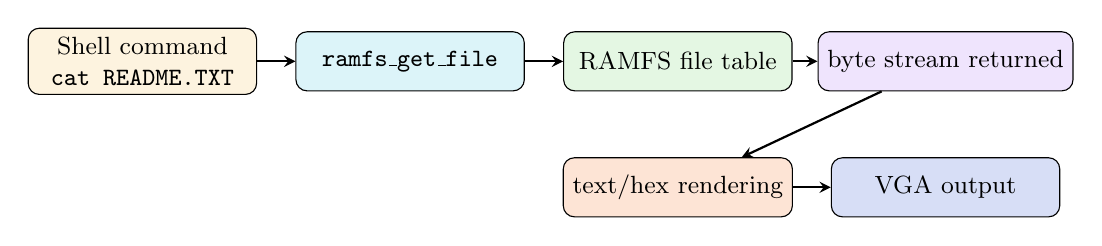
\begin{tikzpicture}[
  box/.style={rectangle,draw,rounded corners=4pt,
    minimum width=2.9cm,minimum height=0.75cm,
    align=center,font=\small},
  arr/.style={->,thick,>=stealth}]

  \node[box,fill=codeyellow!40] (shell) at (0,0) {Shell command\\\texttt{cat README.TXT}};
  \node[box,fill=codeblue!30] (lookup) at (3.4,0) {\texttt{ramfs\_get\_file}};
  \node[box,fill=codegreen!30] (table) at (6.8,0) {RAMFS file table};
  \node[box,fill=codepurple!30] (bytes) at (10.2,0) {byte stream returned};

  \node[box,fill=codeorange!35] (render) at (6.8,-1.6) {text/hex rendering};
  \node[box,fill=codewhite!80] (screen) at (10.2,-1.6) {VGA output};

  \draw[arr] (shell) -- (lookup);
  \draw[arr] (lookup) -- (table);
  \draw[arr] (table) -- (bytes);
  \draw[arr] (bytes) -- (render);
  \draw[arr] (render) -- (screen);
\end{tikzpicture}
\end{center}
\end{frame}

\begin{frame}[fragile]{RAMFS data model}
\begin{lstlisting}[style=clang]
typedef struct {
    const char* name;
    const uint8_t* data;
    uint32_t size;
} ramfs_entry_t;

static ramfs_entry_t g_files[] = {
    {"README.TXT", file_readme, sizeof(file_readme) - 1},
    {"MOTD.TXT", file_motd, sizeof(file_motd) - 1},
    {"KERNEL.CFG", file_kernel_cfg, sizeof(file_kernel_cfg) - 1},
    {"LOGO.BIN", file_logo_bin, sizeof(file_logo_bin)}
};
\end{lstlisting}
\concept{Design choice}{
  Static table keeps behavior deterministic during early-kernel development.
}
\end{frame}

\begin{frame}[fragile]{Lookup API used by shell}
\begin{lstlisting}[style=clang]
int ramfs_get_file(const char* name,
                   const uint8_t** out_data,
                   uint32_t* out_size) {
    for (int i = 0; i < ramfs_count(); i++) {
        if (str_equals(name, g_files[i].name)) {
            *out_data = g_files[i].data;
            *out_size = g_files[i].size;
            return 1;
        }
    }
    return 0;
}
\end{lstlisting}
\end{frame}

\begin{frame}{Shell commands added}
  \small
  \begin{tabular}{@{}p{3.2cm}p{8.8cm}@{}}
    \toprule
    \textbf{Command} & \textbf{Behavior} \\
    \midrule
    \texttt{ls} & lists RAMFS files with byte sizes \\
    \texttt{cat README.TXT} & prints file bytes as text, replacing non-printable bytes with \texttt{.} \\
    \texttt{hexdump LOGO.BIN} & prints offset, hex bytes, and ASCII panel \\
    \bottomrule
  \end{tabular}
\end{frame}

\begin{frame}[fragile]{Hexdump format implementation}
\begin{lstlisting}[style=clang]
for (uint32_t offset = 0; offset < size; offset += 16) {
    print_hex(offset);
    print(": ");
    // 16 hex bytes
    // ASCII side panel
}
\end{lstlisting}
\concept{Why this helps}{
  \texttt{hexdump} is essential when validating binary payloads and corruption cases.
}
\end{frame}

\begin{frame}{Debugging lesson: why dots appeared in \texttt{cat}}
  \begin{itemize}
    \item Symptom: \texttt{cat README.TXT} printed mostly dots instead of text
    \item Cause: bootloader loaded 35 sectors, but kernel image had grown to 36 sectors
    \item Effect: final kernel bytes (including RAMFS data) were not present in memory
    \item Fix: added third CHS read (C1/H0/S1, 1 sector)
  \end{itemize}
  \warn{Low-level storage bugs can look like parsing/rendering bugs at shell level.}
\end{frame}

\begin{frame}[fragile]{Bootloader load-size fix}
\begin{lstlisting}[style=clang]
; read 17 sectors: C0/H0/S2
; read 18 sectors: C0/H1/S1
; read 1  sector : C1/H0/S1
; total = 36 sectors
\end{lstlisting}
\concept{Reliability takeaway}{
  Kernel growth requires matching bootloader load strategy, or runtime data appears corrupted.
}
\end{frame}

\begin{frame}{Keyword glossary}
  \small
  \begin{tabular}{@{}p{3.0cm}p{9.0cm}@{}}
    \toprule
    \textbf{Keyword} & \textbf{Meaning} \\
    \midrule
    \texttt{RAMFS} & In-memory filesystem where file entries and bytes live in RAM. \\
    \texttt{read-only} & Files can be listed/read but not created, modified, or deleted. \\
    \texttt{entry table} & Array of filename, data pointer, and file size metadata. \\
    \texttt{hexdump} & Utility that shows raw bytes in hexadecimal and ASCII side-by-side. \\
    \texttt{CHS} & Cylinder/Head/Sector disk addressing mode used by BIOS reads. \\
    \bottomrule
  \end{tabular}
\end{frame}

\begin{frame}{Module-level changes}
  \small
  \begin{tabular}{@{}p{2.8cm}p{9.2cm}@{}}
    \toprule
    \textbf{Module} & \textbf{Change} \\
    \midrule
    \texttt{ramfs.c/h} & Added filesystem API and static file image \\
    \texttt{shell.c} & Added \texttt{ls}, \texttt{cat}, and \texttt{hexdump} command handlers \\
    \texttt{kernel.c} & Added \texttt{ramfs\_init()} in startup sequence \\
    \texttt{Makefile} & Added RAMFS object compilation and linking \\
    \texttt{bootloader.asm} & Expanded CHS kernel loading to include additional sector \\
    \bottomrule
  \end{tabular}
\end{frame}

\begin{frame}{Validation checklist for this chapter}
  \begin{enumerate}
    \item Run \texttt{ls} and verify all RAMFS filenames and sizes
    \item Run \texttt{cat README.TXT} and confirm readable text lines
    \item Run \texttt{cat MOTD.TXT} and verify expected message output
    \item Run \texttt{hexdump LOGO.BIN} and verify hex+ASCII formatting
    \item Rebuild and reboot; confirm outputs remain stable across runs
  \end{enumerate}
\end{frame}

\begin{frame}{Limits and next evolution}
  \begin{itemize}
    \item Current FS content is compiled into kernel binary (not external image yet)
    \item No write path, allocation map, or directory hierarchy
    \item Next step: block-backed read-only filesystem region on floppy image
    \item After that: writable metadata and file loading for user programs
  \end{itemize}
\end{frame}

\begin{frame}{Outcome}
  \begin{itemize}
    \item MyOS now has a working filesystem abstraction for named file access
    \item Shell supports practical file introspection in text and binary formats
    \item Boot loading was hardened to keep file data reliable at runtime
    \item Platform is ready for block-based FS and program loader stages
  \end{itemize}
  \vspace{8pt}
  \begin{center}
    \Large \textbf{Chapter 8 establishes the first real filesystem milestone.}
  \end{center}
\end{frame}

\end{document}
